\chapter{Pengujian}

Pada bab ini akan dilakukan pengujian untuk melihat efek penerapan metode \textit{clustering} untuk menyaring fitur lokal terhadap ketepatan dan waktu proses BSIS. Pengujian yang dilakukan ini akan menggunakan cara yang sama dengan yang ada pada \ref{sec:analisis_bsis} tetapi dengan menggunakan dataset dan parameter \textit{threshold} yang berbeda. 

\section{Dataset} 
Pengujian akan dilakukan menggunakan dataset berisi gambar-gambar POI. Gambar-gambar tersebut diperoleh dengan mengambil gambar secara langsung dengan kamera dan dengan menangkap layar dari Google Streetview. Secara keseluruhan dataset terbagi menjadi 10 kelas, di mana kelas merupakan sebuah POI. Setiap kelas pada dataset memiliki sebanyak 15 gambar. Gambar-gambar pada kelas yang sama tersebut merupakan gambar dari sebuah POI yang sama yang diambil dari sudut pengambilan dan waktu pengambilan yang berbeda. Beberapa contoh gambar yang digunakan pada dataset ini dapat dilihat pada Gambar~\ref{fig:contoh_dataset_pengujian}.
\begin{figure}[H]
	\centering
	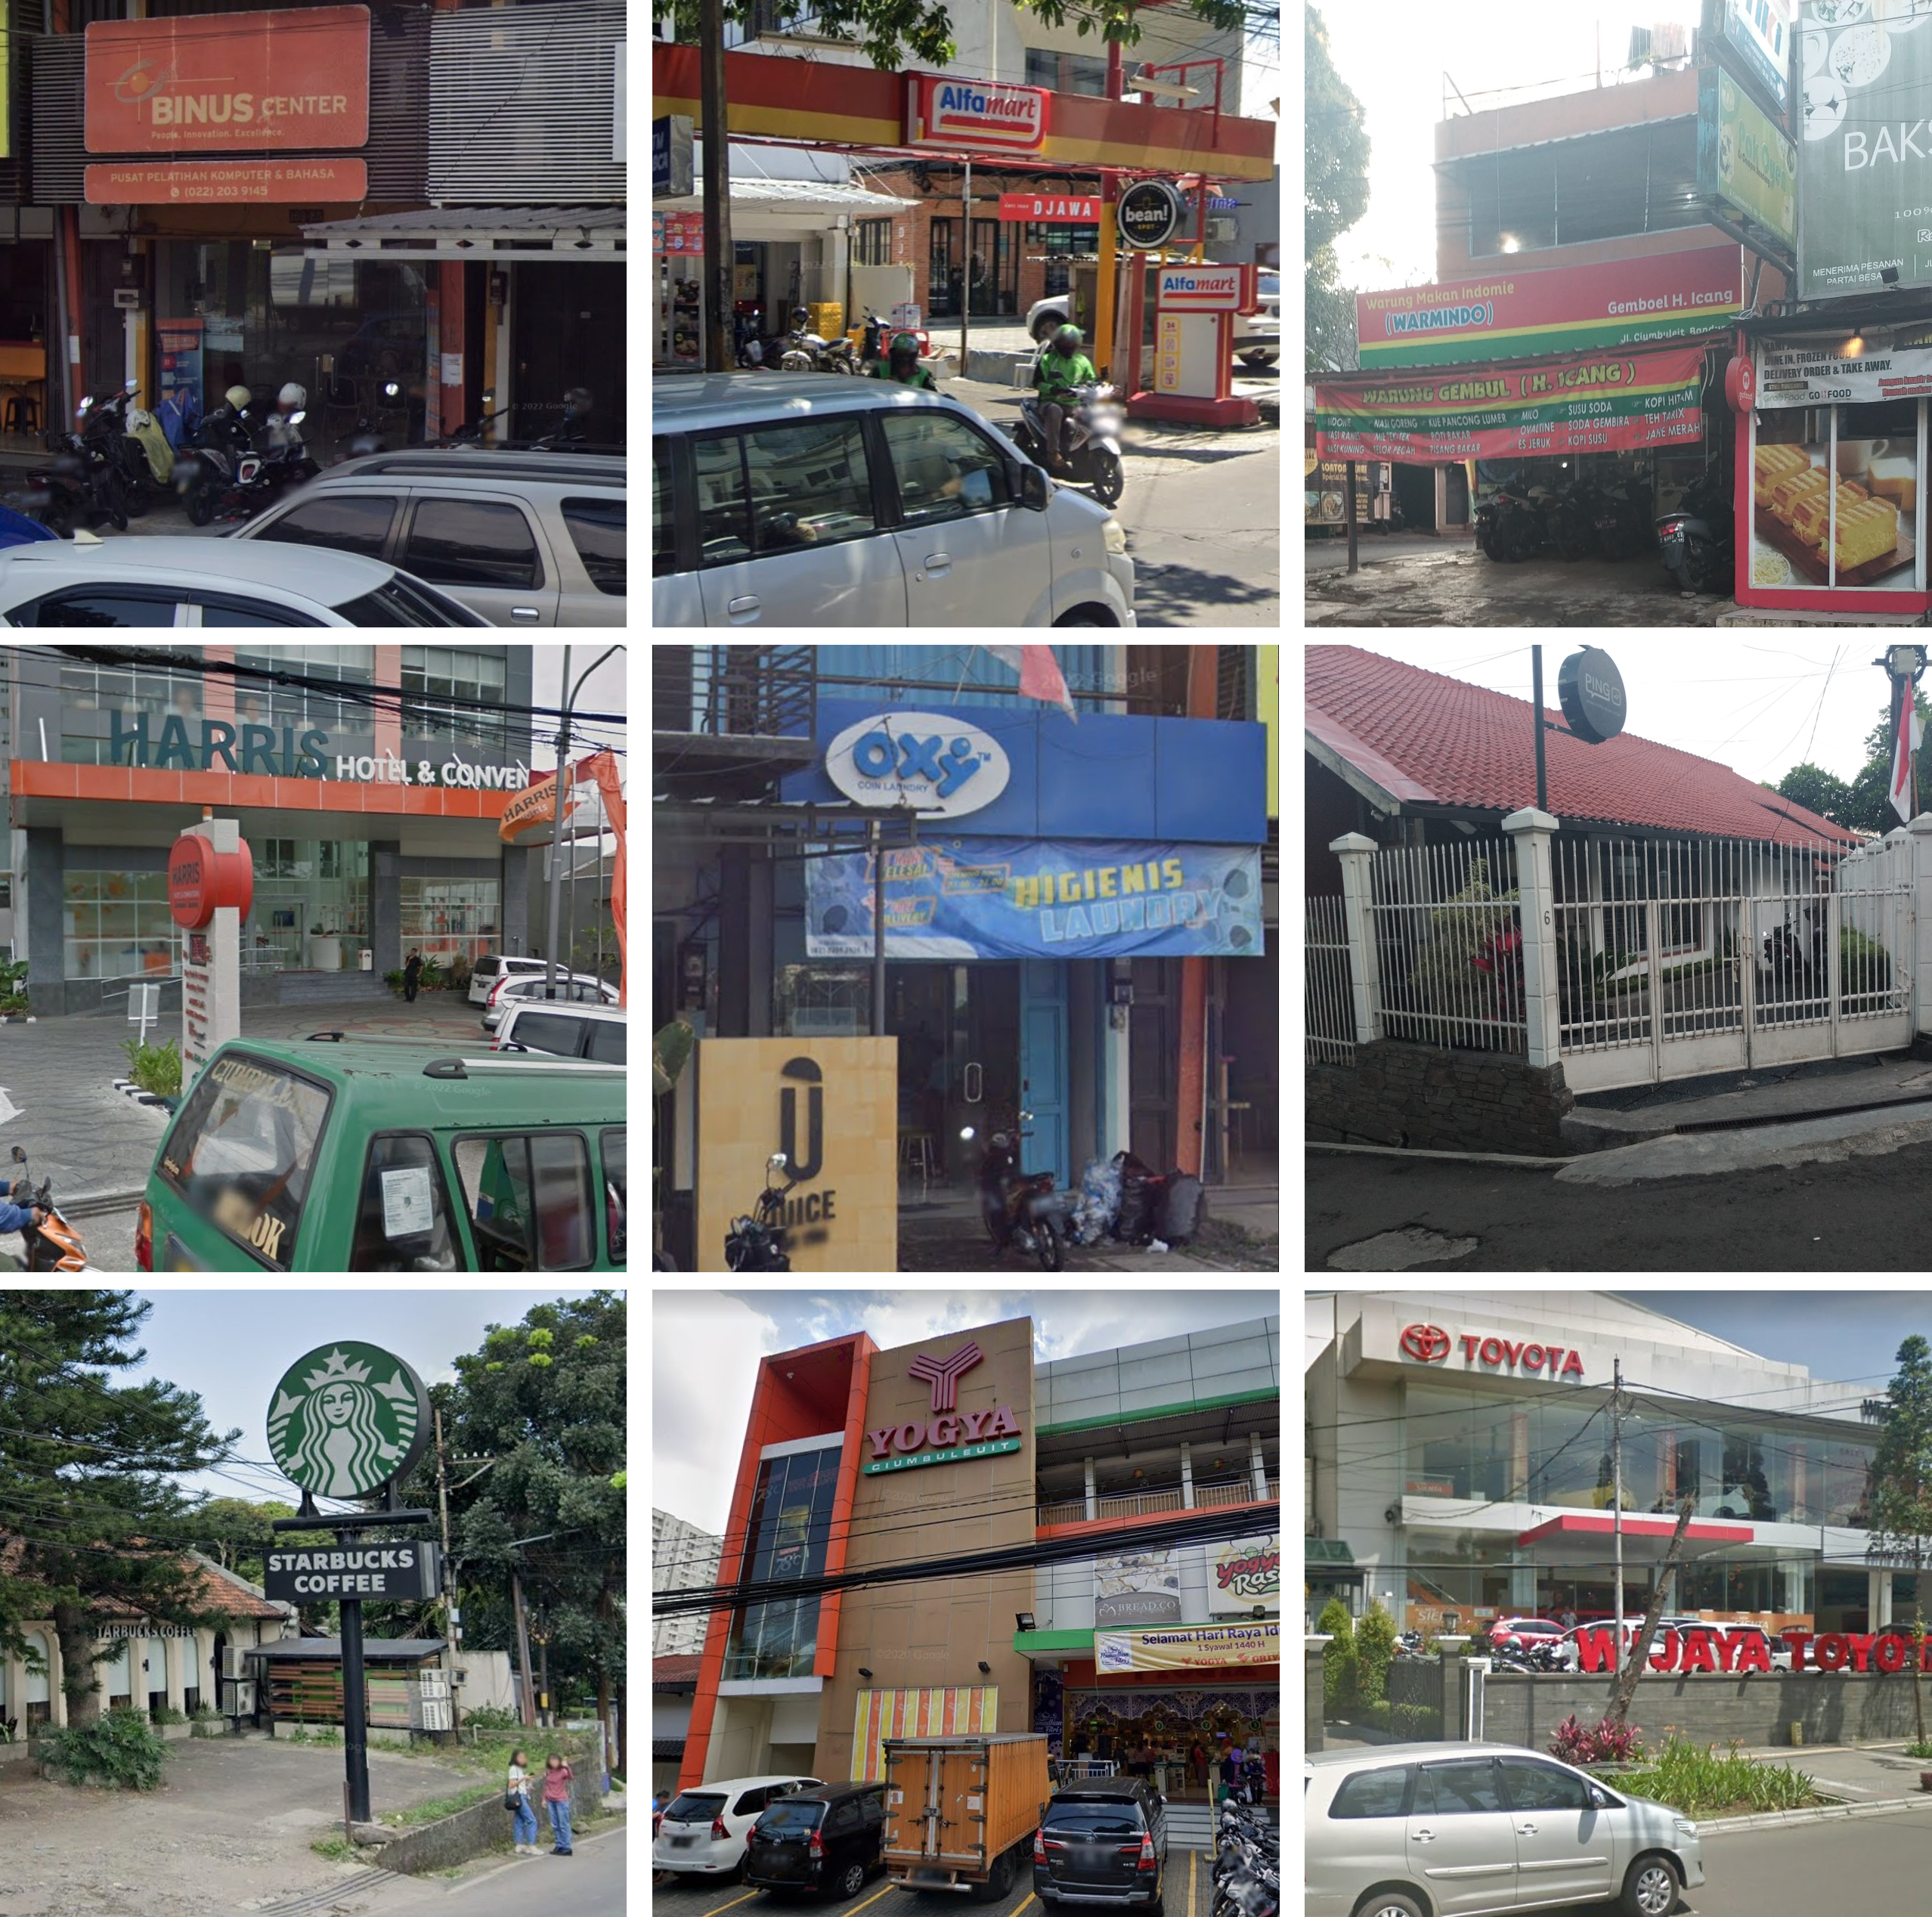
\includegraphics[width=\textwidth]{contoh_dataset_pengujian.png}
	\caption{Beberapa contoh gambar yang digunakan pada pengujian ini.}
	\label{fig:contoh_dataset_pengujian}
\end{figure}

Dataset berjumlah total sebanyak 150 gambar tersebut akan dibagi menjadi data \textit{train} yang digunakan untuk membuat model dan data \textit{test} yang digunakan untuk menguji hasil ketepatan model. Pembagian data menjadi \textit{train} dan \textit{test} akan dilakukan dengan membagi gambar tiap kelas. Untuk setiap kelas akan diambil 10 gambar sebagai \textit{train} dan 5 gambar sebagai \textit{test}. Dengan pembagian seperti demikian maka akan didapat total sebanyak 100 gambar \textit{train} yang terbagi rata menjadi 10 gambar dari tiap kelas, dan 50 gambar \textit{test} yang juga terbagi rata menjadi 5 gambar dari tiap kelas.